% Final STK 795 research report.
% Formatting follows 03_latex_template/legacy_formatting_source.tex (article 10pt, A4,
% margins 3/2.5/2.5/2.5 cm, double spacing, natbib numbers + apalike). Packages that the
% legacy file loaded but this report does not use (pstricks family, babel, rotating, ...)
% are omitted; none of them affects the page layout.
% Build from report/:  latexmk   (settings in latexmkrc; output in build/)
\documentclass[english]{article}
\usepackage[T1]{fontenc}
\usepackage[utf8]{inputenc}
\usepackage[a4paper]{geometry}
\geometry{verbose,tmargin=3cm,bmargin=2.5cm,lmargin=2.5cm,rmargin=2.5cm}
\usepackage{url}
\usepackage{amsmath,amssymb}
\usepackage{graphicx}
\usepackage{booktabs}
\usepackage{setspace}
\usepackage[numbers,sort&compress]{natbib}
\usepackage[hidelinks]{hyperref}
\doublespacing

\graphicspath{{../figures/}}
% Generated table rows (tables/*.tex) are read with the primitive \input so they expand
% inside tabular environments.
\makeatletter
\newcommand{\tabinput}[1]{\@@input #1 }
\makeatother
% Title-page date in the day-month-year form of the legacy template (compile date).
\newcommand{\reportdate}{\number\day\ \ifcase\month\or January\or February\or March\or April\or
  May\or June\or July\or August\or September\or October\or November\or December\fi\
  \number\year}
\newcommand{\T}{^{\mathsf T}}
\newcommand{\ARL}{\mathrm{ARL}}
\newcommand{\SPE}{\mathrm{SPE}}

\begin{document}

\title{One-class hybrid SVM-CAE based MEWMA monitoring scheme}

\author{Stephen Pienaar (u22594583)\vspace{0.5cm}\\
STK 795 Research Report\vspace{2cm}\\
Submitted in partial fulfillment of the degree BCom(Hons) Statistics and Data Science\vspace{0.5cm}\\
Supervisor(s): Dr. MJC Malela, Co-supervisor(s): Dr. Lyson Chaka \vspace{2cm}\\
Department of Statistics, University of Pretoria\vspace{0.5cm}\\

\includegraphics[width=5cm]{UPlogohighres.jpg}\vspace{0.5cm}\\
\reportdate}

\date{}

\maketitle
\newpage{}
\begin{abstract}
This report develops and evaluates a hybrid multivariate monitoring scheme that combines a
one-dimensional convolutional autoencoder (CAE), a one-class support vector machine (OC-SVM) and
a multivariate exponentially weighted moving average (MEWMA) control chart. For every window of
32 observations, the CAE's reconstruction error and the OC-SVM's anomaly score on the CAE
features form a two-dimensional monitoring vector that the MEWMA accumulates over time. The
scheme is studied on a simulated nonlinear process driven by a latent vector autoregression,
using five independent datasets for representation learning, detector fitting, empirical
calibration of the control limit to an in-control average run length (ARL) of 370, independent
in-control validation, and out-of-control evaluation under sustained latent mean shifts of
magnitude 0.2 to 3.0. On independent in-control data the hybrid chart was somewhat more liberal,
and a classical raw-data MEWMA somewhat more conservative, than the design target. Out of control,
the hybrid chart had a shorter average run length than both of its single-component ablations at
every shift, but it did not outperform the classical MEWMA: the two were indistinguishable at the smallest
shift, and the classical chart detected faster at every shift of 0.4 or more. Post-hoc
diagnostics attribute this mainly to the weak response of distance-type learned features to a
directional mean shift, amplified at large shifts by the startup behaviour of the charts.

\end{abstract}

\newpage{}

\section*{Declaration}

I, \emph{Stephen James Pienaar, }declare that this research report, submitted in
partial fulfillment of the degree \emph{BCom(Hons) Statistics and Data Science, }at
the University of Pretoria, is my own work and has not been previously
submitted at this or any other tertiary institution.

\vspace{1cm}

\_\_\_\_\_\_\_\_\_\_\_\_\_\_\_\_\_\_\_\_\_\_\_\_\_\_\_\_\_

\emph{Stephen James Pienaar}

\vspace{1cm}

\_\_\_\_\_\_\_\_\_\_\_\_\_\_\_\_\_\_\_\_\_\_\_\_\_\_\_\_\_

\emph{Dr. MJC Malela}

\vspace{1cm}

\_\_\_\_\_\_\_\_\_\_\_\_\_\_\_\_\_\_\_\_\_\_\_\_\_\_\_\_\_

\emph{Dr. Lyson Chaka}

\vspace{1cm}

\_\_\_\_\_\_\_\_\_\_\_\_\_\_\_\_\_\_\_\_\_\_\_\_\_\_\_\_\_

Date

\newpage{}

\section*{Acknowledgements}

I would like to express my sincere gratitude to my supervisors for their invaluable guidance, support, and encouragement throughout the completion of this thesis. Their expertise and feedback have played an important role in shaping this research. I would also like to thank my family for their continuous support, patience, and encouragement throughout my studies. Their belief in me and constant motivation have been greatly appreciated.

\newpage{}

\tableofcontents{}

\listoffigures

\listoftables

\newpage{}

% ---------------- core report body (exactly 10 pages) ----------------
\section{Introduction}

\subsection{General concepts in SPC and ML}

\subsubsection{Statistical Process Control}

Statistical process control (SPC) is a collection of statistical techniques for monitoring process
stability and improving capability by reducing variability \citep{montgomery_statistical_2012}. Its
principal tool is the control chart, which plots a monitoring statistic against a control limit;
a value beyond the limit signals a possible out-of-control (OOC) departure from the in-control (IC)
state. Charts are judged by their run lengths, usually through the average run length (ARL): a long
in-control ARL ($\ARL_0$) means few false alarms and a short out-of-control ARL ($\ARL_1$) fast
detection \citep{ahmed_statistical_2017}. Memoryless Shewhart-type charts suit large shifts, whereas
memory-type charts such as the cumulative sum (CUSUM) \citep{page_continuous_1954} and the
exponentially weighted moving average (EWMA) \citep{roberts_control_1959} accumulate evidence and
suit small, persistent shifts; the multivariate EWMA (MEWMA) \citep{lowry_multivariate_1992} extends
this to correlated characteristics. These charts assume independent, normally distributed
observations, and when either assumption fails the realised $\ARL_0$ can differ substantially from
its nominal value \citep{lowry_multivariate_1992,ahmed_statistical_2017}.

\subsubsection{Machine Learning}

Machine learning (ML) offers data-driven alternatives that need no parametric process model; because
labelled faults are rare, the relevant methods model normal behaviour only
\citep{pimentel_review_2014}. An autoencoder (AE) is a neural network trained to reconstruct its input
through a low-dimensional bottleneck \citep{hinton_reducing_2006}; trained on normal data, its
reconstruction error measures departure from normal structure. A convolutional autoencoder (CAE) uses
convolutional layers
that extract local patterns from inputs such as short multivariate time-series windows
\citep{lecun_gradient-based_1998,honkela_stacked_2011}. The one-class support vector machine
(OC-SVM), an unsupervised extension of the support vector machine \citep{cortes_support-vector_1995},
estimates a region containing most of the normal data and scores new observations relative to its
boundary \citep{scholkopf_estimating_2001}. On CAE features the two signals are complementary: the
score asks whether a window's representation looks typical, the reconstruction error whether the
network can reproduce the window at all.

\subsection{Problem statement and significance of the study}

Nonlinear relationships, serial dependence and non-normality weaken the distributional basis of
standard control limits \citep{lowry_multivariate_1992,ahmed_statistical_2017}. Learned detectors
can represent such structure, but they are usually applied observation by observation against a
fixed threshold, without accumulating evidence or a run-length interpretation of their alarm rate
\citep{mabu_disaster_2019,biegel_deep_2022,guzman_sidewalk_2026}. This study places CAE
reconstruction information and OC-SVM anomaly-score information inside a memory-type MEWMA chart
and evaluates the result as a control chart: its limit is calibrated to a nominal $\ARL_0$ and its
run lengths are compared with those of a classical MEWMA calibrated to the same target, so any
benefit of learning is judged on the classical chart's own terms.

\subsection{Research aim and objectives}

The aim is to develop and evaluate a hybrid ML-based MEWMA monitoring scheme that integrates a CAE and
an OC-SVM for detecting process shifts in multivariate data. The objectives are to:
\begin{itemize}
\item construct a CAE and OC-SVM hybrid that combines both signals in one monitoring vector;
\item investigate its run-length characteristics, with particular interest in small shifts;
\item evaluate the CAE and OC-SVM components using appropriate diagnostics;
\item compare the hybrid with a classical MEWMA under a common in-control design target;
\item examine a range of shift magnitudes and, in a limited analysis, the smoothing constant; and
\item demonstrate the scheme on simulated multivariate process data.
\end{itemize}

\subsection{Research outline}

The study is confined to unsupervised monitoring of a simulated nonlinear process, so the true state
is always known. It covers Phase~I, in which all components and limits are estimated from in-control
data, and Phase~II, in which the frozen scheme is applied to independent sequences
\citep{ahmed_statistical_2017}. Sections~2--6 present the literature review, methodology, results,
practical application and conclusions.

\section{Literature Review}

Memory-type charting began with the CUSUM of \citet{page_continuous_1954} and the geometric moving
average of \citet{roberts_control_1959}. For several correlated characteristics, two traditions
developed. The first extends univariate charts through Hotelling's $T^2$ statistic, culminating
for the memory-type case in the MEWMA chart, whose limit is set to achieve a specified $\ARL_0$ and
whose ARL depends on a mean shift only through its Mahalanobis distance
\citep{lowry_multivariate_1992}. The second, reviewed by \citet{macgregor_statistical_nodate},
projects the observations onto a few latent variables and monitors two complementary statistics:
$T^2$ on the retained scores and a squared prediction error (SPE) on the residual. Both traditions
rest on linear structure and on independence and normality assumptions whose failure can distort
run-length behaviour \citep{ahmed_statistical_2017}; distribution-free schemes relax the
parametric assumptions \citep{arslan_rankbased_2026}.

Representation learning offers a nonlinear counterpart to the projection step. Autoencoders learn
low-dimensional codes that outperform principal components for dimension reduction
\citep{hinton_reducing_2006}, convolutional autoencoders add locality and weight sharing
\citep{honkela_stacked_2011}, and one-dimensional convolutional networks suit sensor signals when
labelled data are scarce \citep{kiranyaz_1d_2021}. The analogy with latent-variable monitoring is
direct: the autoencoder plays the role of the principal component model and its reconstruction
error that of the SPE. For the latent space, one-class methods model normality when abnormal
examples are too scarce to model \citep{pimentel_review_2014}, and the OC-SVM scores observations
relative to an estimated support boundary \citep{scholkopf_estimating_2001}. Feeding learned
latent codes to an OC-SVM is established practice \citep{alaverdyan_regularized_2020,
pinon_one-class_2023,mabu_disaster_2019}, and \citet{guzman_sidewalk_2026} report that combining
autoencoder reconstruction error with an OC-SVM beats either component alone; all of these detectors,
however, classify each observation against a fixed threshold.

Hybrid ML and SPC research has followed two strands. In the first, a learner operates on charting
statistics while the chart remains classical: convolutional and recurrent networks recognise
control-chart patterns \citep{yu_control_2021}, deep networks and support vector regression model
EWMA-type statistics for censored reliability data \citep{lee_residual_2023,lee_monitoring_2024},
and models trained on classical charting statistics widen the range of detectable shifts
\citep{mukhtiar_enhanced_2025}. These learners need labelled out-of-control examples or a parametric
model from which training data are simulated. In the second strand, representation learning enters
the monitoring statistic itself: \citet{biegel_deep_2022} compute $T^2$ and SPE statistics from a
deep autoencoder's latent representation and reconstruction error on a real sheet-metal forming
process. That approach is unsupervised and acts on process observations, but its statistics are
memoryless and it is assessed by classification metrics rather than run lengths. Within the
literature reviewed, no study combines a CAE reconstruction error with an OC-SVM score on the CAE
representation in a memory-type chart whose limit is calibrated to a nominal $\ARL_0$ and compared
with a classical MEWMA under the same target; this study addresses that gap.

\section{Methodology}

\subsection{Simulated process and study design}

A latent state $z_t\in\mathbb{R}^8$ follows a stable mean-adjusted VAR(1), and the four observed
variables are a nonlinear function of it:
\begin{equation}
z_t=\mu_t+\Phi(z_{t-1}-\mu_{t-1})+\eta_t,\quad \eta_t\sim N(0,0.2I_8);\qquad
x_t=W_2\tanh(z_t)+\varepsilon_t,\quad \varepsilon_t\sim N(0,0.05I_4).
\label{eq:process}
\end{equation}
$\Phi$ is symmetric tridiagonal (diagonal 0.55, adjacent off-diagonals 0.15; spectral radius
$\approx0.832$), $\tanh$ acts componentwise and $W_2$ is a fixed $4\times8$ mixing matrix
(Appendix~\ref{app:model}). Each trajectory starts at $z_0=0$ and discards 500 burn-in steps.
Because the map is nonlinear and $p=4<8$, no linear projection of $x_t$ recovers $z_t$; the latent
state is never supplied to any model. The fault is a sustained latent mean shift
$\mu_t=\delta v$ in the fixed direction $v=(1,1,0,\dots,0)\T/\sqrt2$, starting at the first
retained observation ($\tau=1$), so $\delta$ is the Euclidean size of the shift and every
out-of-control trajectory is post-change from its first observation. Fifteen magnitudes,
$\delta=0.2,0.4,\dots,3.0$, are studied; no other fault type is used.

Five datasets generated from independent random streams have separate roles
(Figure~\ref{fig:pipeline}): D1--D3 fit and calibrate the scheme in Phase~I, after which everything is
frozen and applied unchanged to D4 (independent in-control validation) and D5 (out-of-control
evaluation) in Phase~II.

\begin{figure}[!t]
\centering
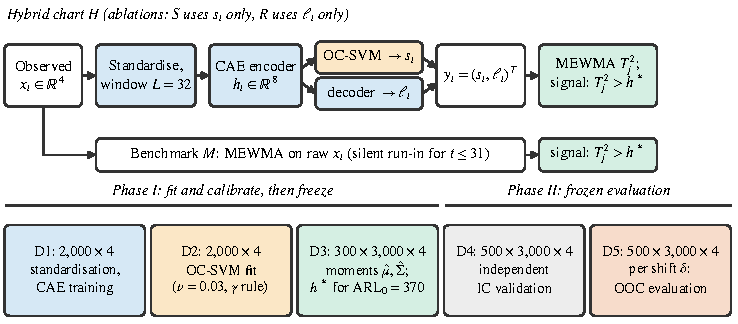
\includegraphics[width=\linewidth]{methodology_pipeline_diagram.pdf}
\caption[Monitoring pipeline and data roles]{Hybrid and benchmark monitoring paths (top) and the
roles of the five datasets (bottom). Box shading marks the dataset on which a stage is fitted or
calibrated; every chart first reports at raw time $t=32$ and has $J=2969$ opportunities per
trajectory.}
\label{fig:pipeline}
\end{figure}

\subsection{Learned components}

\textbf{Windows.} D1 is split chronologically into training rows $[0,1600)$ and validation rows
$[1600,2000)$ before any window is formed. Each variable is standardised with the training-segment
mean and standard deviation, which are then frozen. Windows $X_t\in\mathbb{R}^{4\times32}$ of the
$L=32$ most recent standardised observations are formed with stride 1 inside a segment or
trajectory, so a 3000-observation trajectory yields $J=2969$ windows, the first ending at $t=32$.

\textbf{CAE.} The encoder applies two one-dimensional convolutions ($4\to8\to16$ channels,
kernel 3, stride 2, ReLU), which halve the window length twice ($32\to16\to8$), and a linear
bottleneck producing $h_t\in\mathbb{R}^8$; the decoder mirrors this with a linear layer and two
transposed convolutions (3180 parameters; Appendix~\ref{app:model}). The network was trained on
the 1569 D1 training windows to minimise the mean squared reconstruction error (Adam, learning rate
$10^{-3}$, batch size 64, at most 100 epochs, early-stopping patience 10), and the checkpoint with
the lowest validation loss (epoch 33) was frozen. The reconstruction component is the summed
squared prediction error of the standardised window and its floored logarithm,
\begin{equation}
\SPE_t=\sum_{c=1}^{4}\sum_{k=1}^{32}\big(X_{t,ck}-\hat X_{t,ck}\big)^2,\qquad
\ell_t=\log\max(\SPE_t,10^{-12}).
\label{eq:spe}
\end{equation}

\textbf{OC-SVM.} The 1969 D2 windows are passed through the frozen standardisation and encoder, and
an RBF OC-SVM is fitted to the resulting features directly, without further scaling:
\begin{equation}
k(h,h')=\exp\!\big(-\gamma\lVert h-h'\rVert^2\big),\qquad \nu=0.03,\qquad
\gamma=\Big[\operatorname*{median}_{i<j}\lVert h_i-h_j\rVert^2\Big]^{-1}\approx0.0305,
\label{eq:ocsvm}
\end{equation}
with the median taken over all $\binom{1969}{2}$ pairs. The parameter $\nu$ bounds the fraction of
training windows outside the fitted boundary from above and the fraction of support vectors from
below \citep{scholkopf_estimating_2001}; the fit has 78 support vectors. The monitored score is the
negated decision function, $s_t=\rho-\sum_j\alpha_j k(h_{(j)},h_t)$, so that a larger $s_t$ means a
more abnormal window.

\subsection{Monitoring charts and calibration}

The hybrid monitoring vector is $y_t=(s_t,\ell_t)\T$. For a chart input $u_j$ with in-control mean $\hat\mu$ and covariance $\hat\Sigma$, the MEWMA state
and statistic are \citep{lowry_multivariate_1992}
\begin{equation}
Z_j=\lambda u_j+(1-\lambda)Z_{j-1},\;\; Z_0=\hat\mu,\qquad
T_j^2=(Z_j-\hat\mu)\T(c_j\hat\Sigma)^{-1}(Z_j-\hat\mu),\;\;
c_j=\tfrac{\lambda}{2-\lambda}\big[1-(1-\lambda)^{2j}\big],
\label{eq:mewma}
\end{equation}
where $j$ indexes monitoring opportunities ($j=1$ at $t=32$) and the exact finite-start factor
$c_j$ is always used. Six configurations of four charts are evaluated (Table~\ref{tab:ic}). The
hybrid chart $H$ monitors $y_t$ at the primary $\lambda=0.05$, with $\lambda=0.10$ and $0.20$ as a
sensitivity analysis; the ablations $S$ and $R$ monitor $s_t$ and $\ell_t$ alone, and the benchmark
$M$ is a conventional MEWMA on the raw $x_t$, each with $\lambda=0.05$. $\hat\mu$ and
$\hat\Sigma$ are pooled over all $300\times2969$ D3 monitoring vectors ($S$ and $R$ use the matching
entries) and, for $M$, over the aligned raw D3 observations at $t=32,\dots,3000$. Because the hybrid
charts cannot decide before the first window is complete, $M$'s state is updated silently with
$x_1,\dots,x_{31}$ and it first reports at $t=32$ with factor $c_{32}$, so all six charts share the
same 2969 opportunities.

Consecutive windows share 31 of their 32 observations, so the monitored sequences are strongly
autocorrelated (Section~\ref{sec:components}) and $c_j\hat\Sigma$ is only a reference scaling, not
the covariance of $Z_j$; without independence, limits derived for independent data lose their
nominal ARL properties \citep{lowry_multivariate_1992}. Each limit is therefore calibrated
empirically on D3. For a candidate $h$, $\widehat{\ARL}_0(h)$ is the mean over the 300 D3
trajectories of the first opportunity with $T_j^2>h$, truncated at $J=2969$. As this is a
non-decreasing step function of $h$, the calibrated limit
\begin{equation}
h^*=\min\big\{h\in V:\widehat{\ARL}_0(h)\ge370\big\},
\label{eq:limit}
\end{equation}
where $V$ is the set of values attained by the running maxima of $T_j^2$, is found exactly by
bisection. The target of 370 is the $\ARL_0$ of a conventional three-sigma Shewhart chart
\citep{ahmed_statistical_2017}.

\subsection{Evaluation design}

A run length is the first opportunity $j$ with $T_j^2>h^*$; if none occurs by $j=2969$, the run
length is recorded as 2969 and flagged as censored by a separate indicator, so each mean is a
restricted ARL. D4 yields each chart's independent in-control run lengths, kept distinct from its D3
calibration value, and D5 its out-of-control run lengths at the 15 shifts. Because $\tau=1$, the first window is already post-change and a signal at
opportunity $j$ corresponds to $j+31$ post-change observations: $\ARL_1$ is a detection delay
measured from the first permitted decision, the setting in which \citet{lowry_multivariate_1992}
also compared multivariate charts. $H(0.05)$ and $M(0.05)$ monitor the same D5 trajectories, so the
primary comparison is paired,
\begin{equation}
\bar d(\delta)=\frac{1}{500}\sum_{i=1}^{500}\big[\mathrm{RL}_{H,i}(\delta)-\mathrm{RL}_{M,i}(\delta)\big],
\label{eq:paired}
\end{equation}
with standard error $s_d/\sqrt{500}$; a positive $\bar d$ means that the benchmark signalled first.
The design was fixed in advance: no model, moment, smoothing constant or limit was changed after D4
or D5 was examined.

\section{Results}

Sections~4.1--4.4 report canonical results; Section~4.5 adds post-hoc interpretation.

\subsection{Behaviour of the learned components}
\label{sec:components}

The CAE generalised to independent in-control data, with a mean squared reconstruction error per
window element of 0.66 on the D1 validation windows and 0.67 on D3. The OC-SVM met its
$\nu$-property in sample (3.0\% of D2 windows outside the boundary; 4.0\% support vectors), but
6.2\% of D3 windows fell outside, so its boundary was somewhat tight out of sample, which the
D3-calibrated limit absorbs. Figure~\ref{fig:ic} shows that the components were weakly correlated
($r=-0.15$), that $s_t$ was right-skewed (skewness 0.55) while $\ell_t$ was nearly symmetric, and
that both were strongly serially dependent: their lag-one autocorrelation of 0.96 decayed almost
linearly to near zero at lag 32, where windows stop sharing observations, whereas the raw variables'
lag-one autocorrelations of 0.45--0.60 fell below 0.07 by lag 10. This overlap-induced dependence is
why the limits were calibrated empirically.

\begin{figure}[!t]
\centering
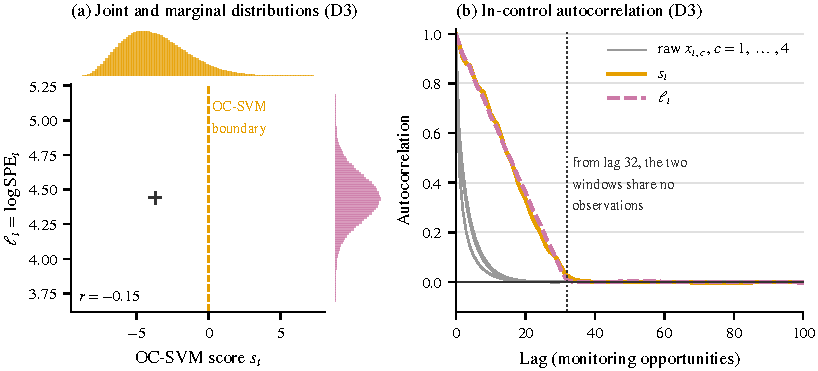
\includegraphics[width=\linewidth]{diagnostic_ic_monitoring_vector.pdf}
\caption[In-control behaviour of the hybrid monitoring vector]{In-control monitoring vectors on
D3 ($300\times2969$ windows, recomputed from the frozen models; they reproduce the stored D3 moments
exactly). (a) Joint distribution of $(s_t,\ell_t)$ (grey shading: log count; cross: $\hat\mu$) with
marginal histograms. (b) Autocorrelation of $s_t$, $\ell_t$ and the four raw variables, pooled over
trajectories.}
\label{fig:ic}
\end{figure}

\subsection{In-control validation}

Table~\ref{tab:ic} sets each chart's D3 calibration value beside its independent D4 performance; no
D4 run length was censored (one D3 trajectory was censored when calibrating $H(0.20)$). The realised
$\ARL_0$ departed from 370 in opposite directions: the hybrid configurations ran shorter
(315.4--336.5, i.e.\ 2.3--4.0 D4 standard errors below target), the ablations stayed close (351.4 and
363.4) and $M(0.05)$ ran longer (403.5, 1.9 standard errors above); on the same D4 trajectories,
$M(0.05)$'s run lengths exceeded those of $H(0.05)$ by 67.0 on average (paired SE 22.2). Deviations
of this size can arise from sampling variability in both the finite calibration bank and D4, but
their direction matters: $H(0.05)$ was the more liberal chart in control, which, if anything,
favours it out of control.

\begin{table}[!t]
\centering
\caption[Calibrated limits and in-control validation]{Calibrated limit, D3 calibration $\ARL_0$ and
independent D4 in-control performance (500 trajectories; SE in parentheses) of the six charts.}
\label{tab:ic}
\begin{tabular}{llrrrrr}
\toprule
Chart & Input & $h^*$ & D3 $\ARL_0$ & D4 $\ARL_0$ (SE) & D4 SDRL & D4 MRL \\
\midrule
\tabinput{tables/ic_validation.tex}
\bottomrule
\end{tabular}
\end{table}

\subsection{Primary comparison: \texorpdfstring{$H(0.05)$ versus $M(0.05)$}{H(0.05) versus M(0.05)}}

Figure~\ref{fig:ooc}(a)--(b) covers the complete shift grid; no D5 run length was censored. At
$\delta=0.2$ the charts were indistinguishable ($\ARL_1$ 282.4 and 285.6; $\bar d=-3.2$, paired SE
15.9). At every $\delta\ge0.4$ the benchmark signalled first on average, by more than ten paired
standard errors (Appendix~\ref{app:results}). The absolute gap peaked at $\delta=0.4$--$0.6$
($\bar d\approx98$--106 opportunities) and then narrowed, while the relative gap widened: $M(0.05)$
signalled at its first opportunity in 41\% of trajectories at $\delta=1.0$ and in essentially all
from $\delta=2.2$, whereas $H(0.05)$ never did so and levelled off near an $\ARL_1$ of 12.5. Counted
in post-change observations ($j+31$), the mean delays were 110 against 43 at $\delta=1.0$ and 44
against 32 at $\delta=3.0$, a ratio of 1.4--2.5 for $\delta\ge0.4$, compared with up to 21 in
monitoring opportunities. Under this sustained directional mean shift, the classical benchmark
therefore detected faster at every shift from 0.4 upwards, despite being the more conservative chart
in control.

\begin{figure}[!t]
\centering
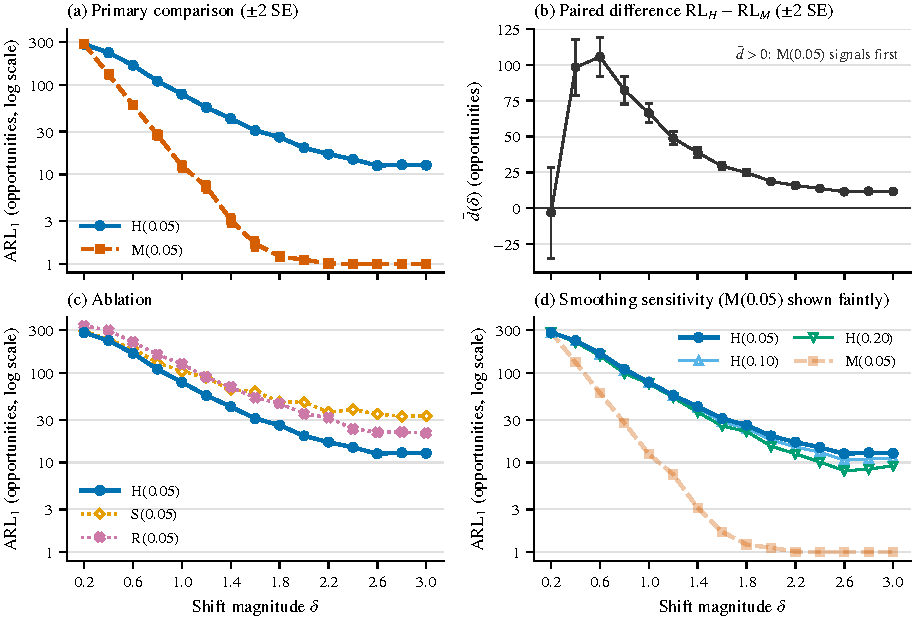
\includegraphics[width=\linewidth]{results_ooc_arl_panels.pdf}
\caption[Out-of-control performance across the shift grid]{Out-of-control results on D5 (500
trajectories per $\delta$; log scale in (a), (c), (d)). (a) $\ARL_1$ of $H(0.05)$ and $M(0.05)$;
(b) paired mean difference $\bar d(\delta)$ of Equation~(\ref{eq:paired}); (c) $H(0.05)$ and its
ablations; (d) the three hybrid smoothing constants, with $M(0.05)$ for reference.}
\label{fig:ooc}
\end{figure}

\subsection{Ablation and smoothing sensitivity}

Figure~\ref{fig:ooc}(c) shows that $H(0.05)$ had a lower $\ARL_1$ than both ablations at all 15
shifts. Paired over the same trajectories (Appendix~\ref{app:results}), its advantage over $R(0.05)$
was clear throughout (8.6--69.0 opportunities, more than three paired SE), whereas that over
$S(0.05)$ was within sampling error at $\delta\le0.4$ ($-9.7$, SE 14.5; $-6.4$, SE 11.3) and exceeded
two paired SE from $\delta=0.6$; the score was the stronger single component up to $\delta=1.4$ and
the reconstruction error beyond it. Figure~\ref{fig:ooc}(d) shows that a larger $\lambda$ changed
little at small shifts and helped at larger ones, as expected for EWMA-type charts
\citep{lowry_multivariate_1992}: $H(0.20)$ had the lowest hybrid $\ARL_1$ at every $\delta\ge0.4$, by
2.6--11.0 opportunities relative to $H(0.05)$. Its D4 $\ARL_0$ was also lower (paired difference
$-21.1$, SE 11.0), so part of this gain may reflect a more liberal realised calibration, and no
smoothing constant in the pre-specified range brought the hybrid close to $M(0.05)$.

\subsection{Interpretation}

Two features of the design explain these results. First, the fault is a sustained mean shift in a
fixed direction, the alternative that a linear, accumulating MEWMA on $x_t$ is built to detect
\citep{lowry_multivariate_1992}, whereas the hybrid accumulates two distance-type summaries of each
window, which respond weakly to small location shifts. Second, with $\tau=1$ the benchmark's first
report already contains 32 accumulated post-change updates, whereas the hybrid's first statistic is
the Mahalanobis distance of a single window, compared with a limit set by the strongly persistent
steady state. Post-hoc diagnostics, which are not part of the pre-specified experiment, support both
explanations: the component means moved by only 0.10--0.21 in-control standard deviations at
$\delta=0.4$ (Appendix~\ref{app:diagnostics}), and a separate diagnostic audit estimated that $y_t$
retains 2--36\% of the raw data's mean-shift information per update, that startup mechanics account
for most of the gap in monitoring opportunities at $\delta\ge1.8$, and that with the change after
100 in-control reports $H(0.05)$ still needed 2.0--2.5 times as many post-change observations as
$M(0.05)$ for $\delta\ge0.6$. These diagnostics explain the canonical result; they do not change it.

\section{Application}

The scheme was evaluated only on simulated data; no industrial or benchmark process, such as the
Tennessee Eastman Process, was monitored in this study. In practice it would be deployed in the same
two phases. In Phase~I, a stable reference period of normal operation is divided chronologically into
three parts that mirror D1--D3: standardisation and CAE training, OC-SVM fitting on the frozen
encoder's features, and estimation of the moments of $y_t$ with empirical calibration of $h^*$ to the
in-control ARL the plant can tolerate. In Phase~II, each new observation completes a window of the 32
most recent standardised observations; one CAE pass and one OC-SVM evaluation give $s_t$ and
$\ell_t$, which update the MEWMA, and a signal prompts investigation rather than automatic correction.
The computation is light: the CAE has 3180 parameters and the OC-SVM 78 support vectors, and the
complete production run of this study (data generation, training, calibration and Phase~II
evaluation of all six charts) took 207 seconds on a single laptop processor thread.

The practical demands are nonetheless real. The reference period must be genuinely in control,
because faults present in it would be learned as normal. The persistent window features make the
first reports after a restart conservative: no in-control D4 trajectory of $H(0.05)$ signalled before
its eleventh report, whereas $M(0.05)$ could signal at its first. Legitimate process changes require
refitting and recalibration on fresh in-control data, and a signal is harder to trace to individual
variables than with a raw-data MEWMA, whose state vector indicates the direction of a shift
\citep{lowry_multivariate_1992}. Above all, the evidence concerns one simulated process and one fault
family, for which the raw-data benchmark was faster; external validation on the Tennessee Eastman
Process or real plant data is needed before industrial use can be recommended.

\section{Conclusion}

\subsection{Summary}

This study developed a hybrid monitoring scheme in which a CAE supplies a reconstruction error and
learned features, an OC-SVM scores those features, and a MEWMA chart accumulates the vector
$(s_t,\ell_t)$. It was implemented on a simulated nonlinear process with five independent datasets,
and every chart was calibrated empirically to an in-control ARL of 370. The learned components
behaved largely as intended, and on independent in-control data the hybrid was somewhat more liberal,
and the classical benchmark somewhat more conservative, than the target. The hybrid had a lower
$\ARL_1$ than both single-component ablations at every shift (within sampling error only against
$S(0.05)$ at $\delta\le0.4$), so the combined vector carries more usable information than either
learned signal alone, but it did not outperform the classical MEWMA: the two were
indistinguishable at $\delta=0.2$, and the benchmark was faster at every larger shift, by up to 106
monitoring opportunities on average, with the hybrid needing 1.4 to 2.5 times as many post-change
observations. Larger smoothing constants shortened the hybrid's run lengths modestly, most in
relative terms at large shifts, without closing the gap.

\subsection{Recommendations}

First, for sustained mean shifts in a moderately nonlinear process, a well-calibrated classical MEWMA
on the raw variables should remain the default, and a learned monitor should be adopted only where it
improves run-length performance against such a benchmark under a common in-control target. Second,
learned reconstruction and one-class information should be monitored jointly rather than separately,
since the joint chart dominated both ablations. Third, charts built on overlapping windows should be
calibrated empirically on the dependent process, with delays reported both in monitoring
opportunities and in post-change observations.

\subsection{Future work}

The hybrid should be evaluated on faults that alter the shape, variability or dependence of the data
(variance changes, sensor faults, drifts and transients), for which distance-type features may be
better suited than for a mean shift, and on larger, more strongly nonlinear processes.
Direction-preserving learned features, dependence-aware finite-start scaling for overlapping windows,
changes that occur during monitoring, and validation on the Tennessee Eastman Process and real plant
data also deserve study.

\label{body-end}
% ---------------- end of core report body ----------------

\newpage
\phantomsection
\addcontentsline{toc}{section}{References}
\bibliographystyle{apalike}
\bibliography{thesis-lib}

\newpage
\appendix
\section{Simulation and model details}
\label{app:model}

Table~\ref{tab:w2} gives the fixed mixing matrix of Equation~(\ref{eq:process}) (full row rank; the
weights of each observed variable have unit norm) and Table~\ref{tab:cae} the layers of the
convolutional autoencoder, both as implemented in the authoritative repository.

\begin{table}[!ht]
\centering
\caption[The fixed mixing matrix]{The fixed $4\times8$ mixing matrix $W_2$, shown transposed: row $k$
holds the weights of $\tanh(z_{t,k})$ in the four observed variables $x_{t,1},\dots,x_{t,4}$.}
\label{tab:w2}
\begin{tabular}{crrrr}
\toprule
$k$ & $x_{t,1}$ & $x_{t,2}$ & $x_{t,3}$ & $x_{t,4}$ \\
\midrule
1 & $-0.60447198$ & $-0.04842081$ & $-0.05518327$ & $-0.04100004$ \\
2 & $-0.06150649$ & $0.36085142$ & $0.45874929$ & $-0.84305316$ \\
3 & $-0.37179578$ & $-0.83557846$ & $-0.21939336$ & $-0.40588165$ \\
4 & $-0.01161746$ & $-0.11135410$ & $-0.17469105$ & $-0.11509976$ \\
5 & $0.05885824$ & $-0.18152197$ & $-0.55464952$ & $0.26627250$ \\
6 & $0.52361117$ & $0.30422580$ & $0.30578469$ & $0.07542546$ \\
7 & $0.45120458$ & $0.15832824$ & $-0.13652085$ & $0.16952036$ \\
8 & $-0.10604239$ & $0.07924137$ & $-0.53672635$ & $-0.06530930$ \\
\bottomrule
\end{tabular}
\end{table}

\begin{table}[!ht]
\centering
\caption[Layers of the convolutional autoencoder]{Layers of the convolutional autoencoder (kernel 3, stride 2 and padding 1 for every
convolution; output padding 1 for the transposed convolutions).}
\label{tab:cae}
\begin{tabular}{llrr}
\toprule
Stage & Layer & Output shape & Parameters \\
\midrule
Input & standardised window $X_t$ & $4\times32$ & -- \\
Encoder & Conv1d $4\to8$, ReLU & $8\times16$ & 104 \\
 & Conv1d $8\to16$, ReLU & $16\times8$ & 400 \\
 & flatten, Linear $128\to8$ (bottleneck $h_t$) & 8 & 1032 \\
Decoder & Linear $8\to128$, ReLU; unflatten & $16\times8$ & 1152 \\
 & ConvTranspose1d $16\to8$, ReLU & $8\times16$ & 392 \\
 & ConvTranspose1d $8\to4$ (reconstruction $\hat X_t$) & $4\times32$ & 100 \\
\midrule
Total & & & 3180 \\
\bottomrule
\end{tabular}
\end{table}

\clearpage
\section{Supplementary component diagnostics}
\label{app:diagnostics}

Figure~\ref{fig:recon} shows a typical in-control window and its frozen-CAE reconstruction: the
decoder reproduces the smooth level structure of each channel but not the high-frequency
variation, which therefore dominates $\SPE_t$. Figure~\ref{fig:response} compares the in-control
distributions of the standardised components with their distributions under three shifts. It is a
post-hoc descriptive diagnostic computed from the first 100 D5 trajectories at each shift with the
frozen models; it was not a pre-specified output of the experiment.

\begin{figure}[!ht]
\centering
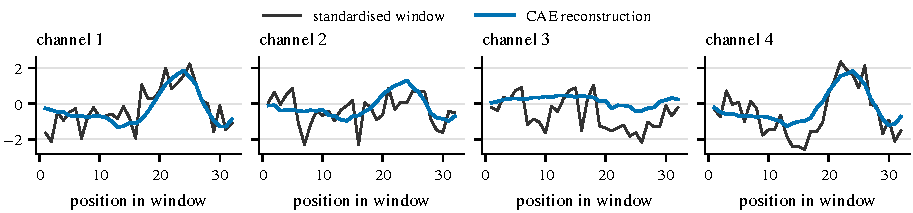
\includegraphics[width=\linewidth]{diagnostic_reconstruction_example.pdf}
\caption[Example window and CAE reconstruction]{One in-control D3 window (trajectory 1, window
1001) and its reconstruction by the frozen CAE ($\SPE_t=96.7$, against a D3 mean of 86).}
\label{fig:recon}
\end{figure}

\begin{figure}[!ht]
\centering
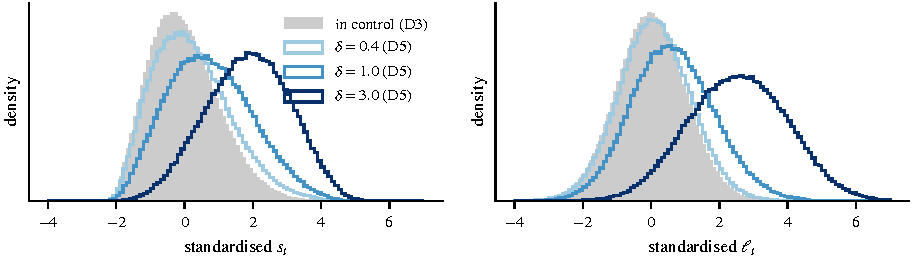
\includegraphics[width=\linewidth]{diagnostic_component_response.pdf}
\caption[Component distributions in and out of control (post-hoc)]{Post-hoc descriptive
diagnostic: distributions of $s_t$ and $\ell_t$, standardised by the D3 moments, in control (D3)
and at $\delta=0.4$, 1.0 and 3.0 (first 100 D5 trajectories each). Mean shifts: $s_t$ 0.21, 0.75,
1.86 and $\ell_t$ 0.10, 0.64, 2.55 standard deviations.}
\label{fig:response}
\end{figure}

\clearpage
\section{Supplementary Phase II results}
\label{app:results}

Figure~\ref{fig:d4} is the repository's own summary of the D4 validation in
Table~\ref{tab:ic}. Tables~\ref{tab:d5}--\ref{tab:ablation} give the complete out-of-control
results; every entry is computed from the committed per-trajectory run lengths, and no D5 run
length was censored. Figure~\ref{fig:boxplots} shows run-length distributions of the primary pair
at four shifts.

\begin{figure}[!ht]
\centering
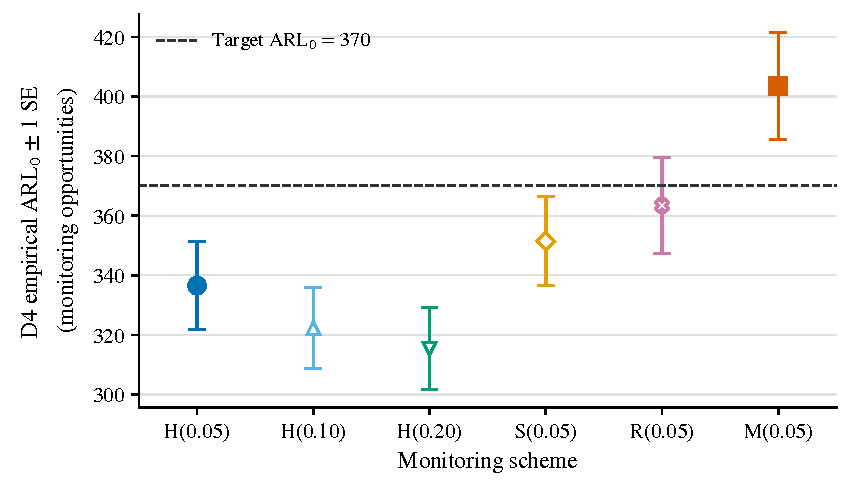
\includegraphics[width=0.7\linewidth]{results_d4_arl0_validation.pdf}
\caption[Independent in-control validation on D4]{D4 in-control ARL ($\pm1$ SE, 500 trajectories)
of the six charts against the target of 370 (repository figure).}
\label{fig:d4}
\end{figure}

\begin{table}[!ht]
\centering
\caption[Out-of-control ARL of all charts]{Restricted out-of-control ARL (SE) of all six charts across the shift grid (D5, 500
trajectories per shift).}
\label{tab:d5}
\small
\begin{tabular}{rrrrrrr}
\toprule
$\delta$ & $H(0.05)$ & $H(0.10)$ & $H(0.20)$ & $S(0.05)$ & $R(0.05)$ & $M(0.05)$ \\
\midrule
\tabinput{tables/d5_arl1_full.tex}
\bottomrule
\end{tabular}
\end{table}

\begin{table}[!ht]
\centering
\caption[Primary paired comparison in detail]{Primary comparison in detail: paired mean difference
$\bar d$ (SE), median run lengths, share of $M(0.05)$ trajectories signalling at the first
opportunity (no $H(0.05)$ trajectory did at any shift), mean delay in post-change observations
($\ARL_1+31$) and the ratio of the two charts' delays in both units.}
\label{tab:primary}
\small
\begin{tabular}{rrrrrrrrr}
\toprule
 & & \multicolumn{2}{c}{MRL} & & \multicolumn{2}{c}{Obs.\ delay} & \multicolumn{2}{c}{Ratio $H/M$} \\
\cmidrule(lr){3-4}\cmidrule(lr){6-7}\cmidrule(l){8-9}
$\delta$ & $\bar d$ (SE) & $H$ & $M$ & $P(\mathrm{RL}_M=1)$ & $H$ & $M$ & obs. & opp. \\
\midrule
\tabinput{tables/primary_contrast.tex}
\bottomrule
\end{tabular}
\end{table}

\begin{table}[!ht]
\centering
\caption[Paired comparison with the ablations]{Paired mean run-length differences (SE) of $H(0.05)$ against its ablations; negative
values mean that $H(0.05)$ signalled sooner.}
\label{tab:ablation}
\small
\begin{tabular}{rrr}
\toprule
$\delta$ & $\mathrm{RL}_H-\mathrm{RL}_S$ & $\mathrm{RL}_H-\mathrm{RL}_R$ \\
\midrule
\tabinput{tables/ablation_contrast.tex}
\bottomrule
\end{tabular}
\end{table}

\begin{figure}[!ht]
\centering
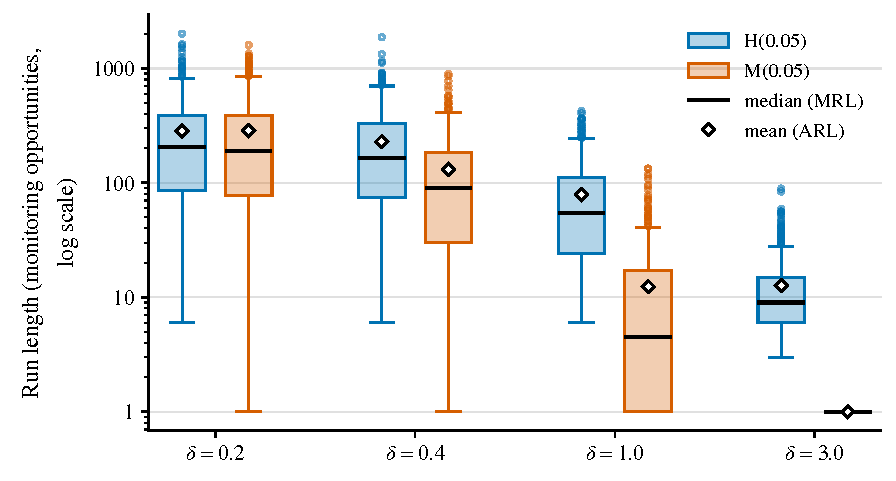
\includegraphics[width=0.8\linewidth]{results_primary_run_length_boxplots.pdf}
\caption[Run-length distributions of the primary pair]{Run-length distributions of $H(0.05)$ and
$M(0.05)$ at four shifts (log scale; repository figure).}
\label{fig:boxplots}
\end{figure}

\clearpage
\section{Reproducibility and provenance}
\label{app:repro}

The experiment is the committed state of the authoritative repository
\texttt{pipeline-thesis-independent} (branch \texttt{simplify-pipeline-code}, commit
\texttt{e62bdee}). Data generation uses master seed 795 with independent PCG64DXSM streams per
dataset, trajectory and shift; the CAE training seed is 3795; all numerical routes run in
double precision (network in single precision) on one CPU thread. The frozen preprocessing
statistics, CAE weights, OC-SVM state, D3 moments and control limits, and the per-trajectory
D4/D5 run lengths are committed artifacts, and the production run that produced them took 207 s.
Every figure and generated table in this report is rebuilt, without refitting or recalibration,
by \texttt{scripts/make\_all\_figures.py} in the report workspace, which reads these artifacts
read-only; the source and derivation of each figure are recorded in
\texttt{provenance/final\_figure\_provenance.md}. The post-hoc diagnostic audit cited in
Section~4.5 is a separate analysis of the same frozen experiment and is not part of its
pre-specified design.


\end{document}
